%! Tex program = xelatex
\documentclass{article}
\usepackage[UTF8]{ctex}
\usepackage{tikz}

\begin{document}

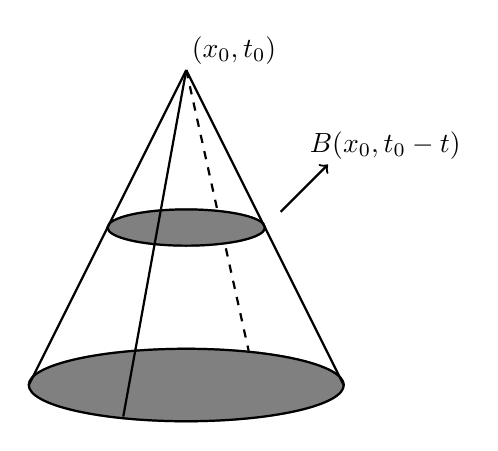
\begin{tikzpicture}[style=thick]
    \draw [dashed] (0,4) -- (0.8,0.4);
    \draw [fill, color=gray] (0,2) ellipse [x radius=1, y radius=0.23]  ;
    \draw [fill, color=gray] (0,0) ellipse [x radius=2, y radius=0.46]  ;
    \draw (0,2) ellipse [x radius=1, y radius=0.23]  ;
    \draw (0,0) ellipse [x radius=2, y radius=0.46]  ;
    \draw (0,4) -- (-2,0);
    \draw (0,4) -- (2,0);
    \draw (0,4) -- (-0.8,-0.4);
    \draw (0,4)[above right=-1.75pt] node{$(x_0,t_0)$};
    \draw [->] (1.2,2.2) -- (1.8,2.8);
    \draw (1.5,2.8)[above right=-1.75pt] node{$B(x_0,t_0-t)$} ;
\end{tikzpicture}

\end{document}